\documentclass{tufte-handout}

\input{vc}

\usepackage{tikz}\usetikzlibrary{decorations.pathreplacing,matrix}

\usepackage{tipa}
\usepackage{color}
\usepackage{listings}
\usepackage{amsmath}

\usepackage[lastexercise,answerdelayed]{exercise}
\setlength{\Exesep}{1ex}
\setlength{\Exetopsep}{1em}
\renewcommand{\ExerciseListName}{Exercise}
\renewcommand{\AnswerListName}{}
\renewcommand{\ExerciseHeaderTitle}{(\emph{\ExerciseTitle.})\ }
\renewcommand{\ExerciseListHeader}{\ExerciseHeaderDifficulty%
\textbf{\ExerciseListName\ExerciseHeaderNB.}\ \ExerciseHeaderTitle%
\ExerciseHeaderOrigin\ignorespaces}
\renewcommand{\AnswerListHeader}{\textbf{\ExerciseHeaderNB.\ }}

\title{Some Useful Math for BADS}
\author{Thore Husfeldt}

\begin{document}
\maketitle
\begin{abstract}
  This note covers some of the mathemematical preliniaries needed to
  enjoy [SW], the textbook \emph{Algorithms, 4th ed.} by Sedgewick and
  Wayne.
\end{abstract}

\section{Some functions encountered it the analysis of algorithms}
\label{sec-1.1}

\subsection{Exponentiation}

For a positive integer $n$ (\emph{the exponent}) and a positive real
number $b$ (\emph{the base}) we define a shorthand for iterated
multiplication, called exponentiation:
\[ b^n = \underbrace{b\times b\times \cdots\times b}_{n \text{ times}}\,.\] 
(Most of the time $b$ will just be $2$, sometimes it's $10$. In maths
and physics, it's often the number $e=2.71\ldots$ and one then uses
the notation $\exp(n)$ for $e^n$, called \emph{the exponential function}.)


\begin{marginfigure}
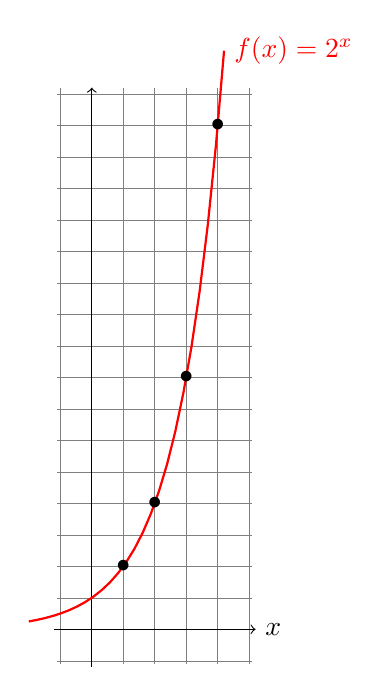
\begin{tikzpicture}[domain=-2:5, scale=.4]
  \draw[very thin,color=gray] (-1.1,-1.1) grid (5.1,17.2);
  \draw[->] (-1.2,0) -- (5.2,0) node[right] {$x$}; \draw[->] (0,-1.2) -- (0,17.2);
  \draw[domain=-2:4.2, thick,red] plot (\x,{pow(2,\x)}) node[right] {$f(x) = 2^ x$};
  \node at (1,2) {$\bullet$};  
  \node at (2,4) {$\bullet$};
  \node at (3,8) {$\bullet$};
  \node at (4,16) {$\bullet$};
\end{tikzpicture}
\end{marginfigure}

\begin{ExerciseList}
\Exercise True or false: $b^{nm}=b^n+b^m$ for $n,m\geq 1$.
\Exercise True or false: $b^{n+m}=b^nb^m$ for $n,m\geq 1$.
\Exercise True or false:  $b^{n-m}=b^n/b^m$ for $n,m\geq 1$.
\Exercise True or false: $(ab)^{n}=a^n+b^n$ for $n\geq 1$.
\Exercise True or false: $(ab)^{n}=a^nb^n$ for $n\geq 1$.
\Exercise True or false: $(a+b)^{n}=a^n+b^n$ for $n\geq 1$.
\Exercise True or false: $(b^n)^m=b^{nm}$ for $n,m\geq 1$.
\Exercise What would be a useful convention for what $b^0$ should
mean?
\Exercise Express as a power of $2$: $2\cdot 2^2$, $(2^2)^3$,
$2^{(2^2)}$, $2^n+ 2^n$.
\end{ExerciseList}

There is a way to define what $b^x$ should mean even when $x$ is
negative, or not even an integer, so that $x\mapsto b^x$ becomes a
smooth function defined for all reals that agrees $b^n$ when $x=n$ is
an integer.  This definition requires calculus and lies outside of our
scope.  The notation makes good sense all the way, for example
$b^{-1}$ equals $1/b$ so that $b^{N+1}b^{-1}= b^N$, and 
$b^{\frac{1}{2}}$ equals  $\sqrt b$ so that
$(b^{\frac{1}{2}})^2 = b^{\frac{1}{2}\cdot 2} = b$.

\subsection{Positional notation}

One of Civilisation's big breakthroughs is to use exponentiation to
denote numbers is a very compact way. When we write 7143 we mean \[
7\cdot 10^3 + 1\cdot 10^2 + 4\cdot 10^1 + 3\cdot 10^0 \,.\]
To see how clever this is, compare to the notation used in ancient Rome
(MMMMMMMCXLIII), or worse, to unary notation. 
Our notation is called ``digital'' or ``base 10'' (because
$b=10$). \marginnote{{\bf digit}, noun, from Latin \emph{digitus}
  'finger, toe'. 1. Any of the numerals $0$ to
  $9$. 2. A finger or toe.}
Positional notation is particularly clever when performing
arithmetic, 
and many people are comfortable using this, having been trained to find
even complicated operations like $100-1=99$ natural. (Compare to the
more straightforward $\mathrm{C}-\mathrm{I} = \mathrm{IC}$.)

\begin{marginfigure}
\begin{verbatim}
0 000
1 001
2 010
3 011
4 100
5 101
6 110
7 111
\end{verbatim}
\end{marginfigure}

\emph{Binary} notation is the positional number system using the base
$b=2$.
It has only two numerals (sometimes also called ``digits'' or ``binary
digits''), $0$ and $1$.
The binary number $1001001$ has value ,
which happens to be 7143 in base 10. 

Just like base 10 makes powers of 10 look good, binary notation makes
powers of 2 look good. \marginnote{There are only 10 kinds of
  people. Those who understand binary and those who don't.}

\begin{ExerciseList}
\Exercise
Express 8 in binary. What is $10010_2$?
\Exercise Add $100101$ and $001011$ using the school algorithm for
addition.
\Exercise Multiply $100101$ and $001011$ using the school algorithm for multiplication.
\end{ExerciseList}


\subsection{Logarithms}

\begin{marginfigure}
\begin{tikzpicture}[domain=-2:4, scale=.8]
  \draw[very thin,color=gray] (-0.1,-1.1) grid (3.9,3.9);
  \draw[->] (-0.2,0) -- (4.2,0) node[right] {$x$}; \draw[->] (0,-1.2) -- (0,4.2) node[above] {$f(x)$};
\draw[domain=.1:4, thick] plot (\x,{ ln(\x)/ln(2)}) node[right] {$f(x) = \lg x$};
\draw[domain=-2:3, thick] plot (\x,{pow(2,\x)}) node[right] {$f(x) = 2^ x$};
\end{tikzpicture}
\end{marginfigure}

The \emph{binary logarithm} $\lg N$ is defined for every positive real
number $N$ and satisfies $2^{\lg N} = N$. Roughly,
``how often you need to double 1 to get $N$.''

More generally, the \emph{logarithm base $b$} for any real $b>1$ is a
function defined for all positive reals $N$ by $\log_b N
= x$ where $b^x= N$.  (To see that this does indeed define $\log_b N$
uniquely we would need to observe that $x\mapsto b^x$ is a bijection
from the reals to the positive reals for $b> 1$. But at this point
we have stopped pretending to give a rigorous presentation anyway.)

Note that $\log_1 5$ or $\lg 0$ and $\lg -1$ are just meaningless collections of
ink, like $8+\times$ or $\frac{\sqrt{} }{4}$.

\begin{ExerciseList}
\Exercise What is $\lg 2$? What is $\log_b b$?
\Exercise What is $\lg 2^x$? What is $\log_b b^x$?
\Exercise True or false: $\log_b (NM)= \log_b N + \log_b M$.
\Exercise True or false: $\log_b (N^x)= x\log_b N.$
\Exercise True or false: $\log_b (N+M)= (\log_b N)( \log_b M)$.
\Exercise Show $\log_a N = \log_b N / \log_b a$.
\Exercise Find $\lg 1024$, $\lg \frac{1}{4}$, $\lg 8$.
\end{ExerciseList}


\subsection{Floors and ceilings}

The \emph{floor function} $\lfloor x\rfloor$ maps any real number $x$
to the largest integer less than or equal to $x$. Likewise, the
\emph{ceiling function} $\lceil x\rceil$ maps any real number $x$ to
the smallest integer greater than or equal to $x$.

\begin{ExerciseList}
\Exercise Find $\lfloor \frac{1}{2}\rfloor$, $\lfloor
  -\frac{1}{2}\rfloor$,  $\lfloor \pi\rfloor$, $\lfloor 7\rfloor$.
\Exercise Find $\lceil \frac{1}{2}\rceil$, $\lceil
  -\frac{1}{2}\rceil$,  $\lceil \pi\rceil$, $\lceil 7\rceil$.
\Exercise Find
 $\lfloor \frac{1}{2}+\lceil \frac{3}{2}\rceil \rfloor$, 
 $\lfloor \frac{1}{2}\cdot \lceil \frac{5}{2}\rceil \rfloor$.
\Exercise For real $x$, true or false: $x-1<\lfloor x \rfloor \leq x \leq
  \lceil x\rceil < x+1$.
\Exercise For all real $x$, true or false: $\lceil -x\rceil = -\lfloor x\rfloor$,
  $\lfloor -x\rfloor = -\lceil x\rceil$.
\Exercise For reals $x$ and $y$, true of false: $\lceil x+y\rceil = \lceil
  x\rceil + \lceil y\rceil$. $\lceil xy\rceil =\lceil x\rceil \lceil
  y\rceil.$
  \Answer False, set $x=\frac{1}{4}, y=3$.
\Exercise For real $x$ and integer $n$, true or false:
  $\lfloor x+n\rfloor = \lfloor x\rfloor+n$,
  $\lceil x+n\rceil = \lceil x\rceil+n$,
\end{ExerciseList}

A particularly interesting function is $\lfloor \log_b N\rfloor$, the
largest integer not greater than $\log_b N$.  This is 1 more than the
number of bits needed to express $N$ in base $b$. For example, in base
$b=10$ we need $\lceil \log_{10} 99\rceil +1= 2$ digits to express
$99$. (In other words, $\lfloor \log_{10} N\rfloor$ function is
\emph{really easy} to compute in your head. Just count the number of
digits and subtract 1. It's one of the most natural properties of a
number. Similarly, if the number is written in binary, $\lfloor \lg N\rfloor$ is
just the number of bits.)

\begin{ExerciseList}
\Exercise How often can you divide a number $N$ by two until you reach $1$
  or less?
\end{ExerciseList}

\subsection{Factorials}

The factorial function is another iterated multiplication, defined for
integer $N\geq 1$ as $N!= N\times (N-1)\times \cdots \times 1$. By
convention, $0!=1$.


\begin{ExerciseList}
\Exercise How big is $N!$ compared to $2^N$ and $N^N$?
\Exercise Find $N$ such that $N!$ is roughly the number of elementary
  particles in the universe.
\Exercise Find $N$ such that $N!$ is roughly the number of nanoseconds
  since the beginning to Time.
\end{ExerciseList}

Except for ``fricking' huge'' it's difficult to get a feeling for the
value of $N!$. A sometimes useful fact, the proof of which is beyond
the scope of this note, is Stirling's approximation,
\[ N! \sim \sqrt{2\pi N} \bigl(\frac{N}{e}\bigr) ^N\,.\]


\subsection{Binomial coefficients}

The number of $k$ element subsets of $\{1,\ldots, N\}$ is denoted
$C(N,k)$. Note that we are talking about sets, and remember that the sets
$\{1,2,4\}$ and $\{1,4,2\}$ are the same. 
For $N=3$ and $k=2$ there are 3 such
sets:
\[ \{1,2\}, \{2,3\}, \{1, 3\}\,.\] A confusing
way\marginnote{Nevertheless, many textbooks use this.} to define
$C(N,k)$ is to say ``the number of ways to pick $k$ elements from
$N$''. I find this confusing because we're \emph{not} actually
interested in the fact that $\{1,2\}$ can be picked in two ways
(``first pick $1$, then $2$'', or ``first pick $2$, then $1$''.)

By contrast, consider number ordered sequences of $k$
elements from $\{1,\ldots, N\}$. For $N=3$ and $k=2$,
\[ (1,1), (1,2), (1,3), (2,1), (2,2), (2,3),(3,1), (3,2), (3,3)\,.\]
In general, there are $N^k$ such sequences, so this number does not
deserve special notation.

\begin{ExerciseList}
\Exercise  Which values do $(r,s,t)$ take? What is the final value of
$C$ in terms of $N$?
\begin{quote}
\begin{lstlisting}[basicstyle=\ttfamily\small]
C = 0
for (int r = 0; r < N; r++)
    for (int s = 0; s < N; s++)
        for (int t = 0; t < N; t++)
            C++;
\end{lstlisting}
\end{quote}
\Exercise Which values do $(r,s,t)$ take? What is the final value of
$C$ in terms of $N$?
\begin{quote}
\begin{lstlisting}[basicstyle=\ttfamily\small]
C = 0
for (int r = 0; r < N-2; r++)
    for (int s = r+1; s < N-1; s++)
        for (int t = s+1; t < N; t++)
            C++;
\end{lstlisting}
\end{quote}
\end{ExerciseList}

Popular notation is $C(N,k)=\binom{N}{k}$. We'll stick to that. 
By
convention, we agree that the number of ways to pick $0$ elements is $1$
(namely ``by not doing anything''), so $\binom{N}{0}= 1$.
You can't pick a nonempty set from an empty set, so $\binom{0}{k}=0$ for
$k\geq 1$.
And, perversely but consequently, $\binom{0}{0}=1$.
These
conventions turn out to lead to pleasant notation and are consistent
with our other choices, such as $0!=1$.

The numbers also appear as coefficients in the evaluation of
binomials, which are expressions of the form $(x+y)^N$. For example
in $(x+y)^2= x^2 + 2xy = y^2$, the coefficients are $1=\binom{2}{0}$, $2=\binom{2}{1}$, and
$1=\binom{2}{0}$. In general, we have the Binomial Theorem,
\[ (x+y)^N = \binom{N}{0} x^N y^0 +\binom{N}{1} x^{N-1}y^1+\cdots
+ \binom{N}{k} x^{N-k}y^k +\cdots+ \binom{N}{N-1} x^1y^{N-1} +
\binom{N}{0} x^0y^N\,.\] 
This is why $\binom{N}{k}$ is often called a \emph{binomial coefficient}.

\begin{ExerciseList}
  \Exercise Find the values $\binom{3}{0}$, $\binom{3}{1}$,
  $\binom{3}{2}$, and $\binom{3}{3}$ by factoring out $(x+y)^3$.
  \Exercise Find $\binom{N}{0}+\binom{N}{1}+\cdots+\binom{N}{N}$.
  \Answer Plug $x=y=1$ into the Binomial Theorem and watch. For a
  combinatorial argument, the sum describes the number of a ways to
  pick a $k$-element set from $\{1,\ldots, N\}$. Since we're summing
  over all $k$, this counts the number of ways to pick a subset of any
  size. There are $2^N$ subsets.
\end{ExerciseList}

One can give a closed formula for $C(N,k)$ in terms of factorials:
\[ \binom{N}{k}= \frac{N!}{k!(N-k)!}\,. \] 
This formula is surprisingly
useless both for getting an intuition about the size of $\binom{N}{k}$ and
for actually computing it (because the numbers are so huge).
Still, it's good enough for some small numbers:

\begin{ExerciseList}
  \Exercise Express $\binom{N}{1}$, $\binom{N}{2}$, and
  $\binom{N}{3}$ as polynomials in $N$.
\end{ExerciseList}

\subsection{Harmonic numbers}

[To be written]

\end{document}
